\Chapter{2次元座標系と地図投影法パラメタ}
\label{chap:proj}

\newcommand{\DP}[2]{\frac{\partial{#1}}{\partial{#2}}}%

\section{概要}

種別1の5文字目と6文字目は
NuSDaS のデータ記録が持つ2次元格子と空間位置との対応関係を表わす。
水平2次元格子について
この関係が数式で書けるようなものの場合、
地図投影法 map projection ともよばれる。

以下の説明ではデータ記録の格子点が
$(1, 1)$, $(1, 2)$, ... $(1, N_X)$, $(2, 1)$, $(2, 2)$, ... $(N_X, N_Y)$
という格子番号 $(i, j)$ をもつものとする。
水平格子では
$(i, j)$ から地球上の経緯度 ($\lambda, \varphi$)
を与える写像がわかれば、
与えられた NuSDaS データの各格子が表現する位置を知ることができることになる。

地図投影では説明の便宜上、
経緯度から必ずしも整数でない格子位置 $x$, $y$ を求める式を紹介するが、
各格子点から経緯度を求める際にはこの逆写像%
\footnote{必ずしも解析的に求められるとは限らない}
\(\lambda(x, y)\),
\(\varphi(x, y)\)
に
\(x = i\), \(y = j\)
を与えれば経緯度を得ることになる。

気象用途で用いられる地図投影法は地図学で考案されたものが
何でも用いられるわけでなく、
数値予報モデルを構成するときの式変形の便宜、
また天気図などの図形表現が歪まないようにするためなどの目的から
正角 (または等角) 図法 conformal projection すなわち
経線・緯線がどこでも直交し (次の \ref{eq:cvlinear.normal})、かつ
方向によって局所的縮尺が異ならない (\ref{eq:conformal})
ものだけが用いられる。
%
\begin{eqnarray}
 \DP{\lambda}{x}\DP{\varphi}{x} + \DP{\lambda}{y}\DP{\varphi}{y} &=& 0
 \label{eq:cvlinear.normal}
\\
 \left(a\cos\varphi\DP{\lambda}{x}\right)^2 + \left(\DP{\varphi}{x}\right)^2
 &=&
 \left(a\cos\varphi\DP{\lambda}{y}\right)^2 + \left(\DP{\varphi}{y}\right)^2
 \label{eq:conformal}
\end{eqnarray}
%
ここで $a$ は地球半径である。
斜軸ランベルト以外では地球を球体としており、
原則として日本測地系 2000 で用いる GRS80 楕円体の平均半径
6371\,000 m が用いられる。

\section{経緯度座標 (LL)}

\paragraph{表式}
経緯度座標は格子番号と経緯度に次のような線形関係があるものである%
\footnote{
地図学上は正距円筒図法 equidistant cylindrical projection あるいは
正方形図法 equirectangular projection 仏 plate care\'e と呼ばれる。
なお、自明とは思うがこの図法は直交だが正角ではない。
}
%。
\begin{eqnarray}
 \lambda &=& \lambda_0 + (i - i_0) D_i
\\
 \varphi &=& \varphi_0 - (j - j_0) D_j
\end{eqnarray}
ここで $D_j > 0$ は北から南の順で格納することを意味することに注意されたい%
\footnote{南から北の順で格納するためには $D_j < 0$ とするが、現在用例はない。}%
。

\paragraph{定義ファイル}
各定数は
格子間隔 ($D_i, D_j$; 度単位), 参照格子点 ($i_0, j_0$),
参照点の経緯度 ($\lambda_0, \varphi_0$; 度単位)
と呼ばれ、次のように定義ファイルに書かれる:
\begin{quote}
\begin{tabular}{lllll}
{\tt distance}	& $D_i$ & $D_j$ & & \\
{\tt basepoint}	& $i_0$ & $j_0$	& $\lambda_0${\tt E} & $\varphi_0${\tt N} \\
\end{tabular}
\end{quote}
参照点 $(i_0, j_0)$ は通常 (1, 1) が用いられる。
たとえば全球 1.25 度格子ならば次のようである:
\begin{screen}
\begin{verbatim}
size       288  145
basepoint  1    1    OE   90N
distance   1.25 1.25
\end{verbatim}
\end{screen}

\paragraph{パラメタの許容範囲}
写像が出来るための数学的制約は
\( D_i \ne 0 \),
\( D_j \ne 0 \)
だけであるが、常識的に
\( -180^\circ < D_i < 180^\circ \),
\( -180^\circ < D_j < 180^\circ \),
書法上
\( -180^\circ < \lambda_0 \le 180^\circ \),
\( -90^\circ \le \varphi_0 \le 90^\circ \),
が要請される。

\section{矩形ガウス格子 (GS)}

\paragraph{表式}
矩形ガウス格子 Gaussian grid%
\footnote{おそらく気象界でしか通用しない用語}
は経緯度座標に似ているが、
$y$ 方向の格子点がルジャンドル多項式 $P_n(\sin\varphi)$ の零点に
とられる点が異なる。

ルジャンドル多項式は帯球関数とも呼ばれるもので
\begin{eqnarray}
 P_n(\mu) &=& \frac{1}{2^nn!}\frac{d^n}{dx^n} (\mu^2 - 1)^n
\\
 &=& \sum_{s=0}^{s \le {n\over 2}}
 	(-1)^s
	\frac{(2n - 2s)!}{2^n s! (n - s)! (n - 2s)!}
	\mu^{n - 2s}
\end{eqnarray}
などで与えられる \(\mu = \sin\varphi\) について $n$ 次の多項式で
\(-1 \le \mu \le 1\)
の間に $n$ 個の零点を持つ\cite[第10章]{terakan}。

\paragraph{定義ファイル}
この格子系は球面調和関数による直交関数展開を用いる
全球スペクトルモデルで用いられ、このとき $n$ は偶数である。
経緯度格子の東西軸の情報に加えて
ルジャンドル多項式の次数 (モデルの切断波数) $n$ が
わかれば格子位置がわかるため
定義ファイルでは次のように記述する:
%
\begin{quote}
\begin{tabular}{lllll}
{\tt distance}	& $D_i$ & $D_j$ & & \\
{\tt basepoint}	& $i_0$ & $j_0$	& $\lambda_0${\tt E} & {\tt 0.0N} \\
{\tt standard}	& $n${\tt E} & {\tt 0N} & {\tt 0E} & {\tt 0N} \\
\end{tabular}
\end{quote}
%
ここで $j_0$ は赤道に対応する格子番号 $j$ (2格子の中点なので半奇数)
であり、
全球モデルから得られた全格子ならば
\(
	D_i = 360^\circ/(2n),
\)
\(
	j_0 = (n + 1)/{2}
\)
である。
なお、$D_j$ には $D_i$ と同じ値を書くが、
これは平均的な南北方向の格子間隔をおおざっぱに示したものである。
次の例は $T_L319$ のガウス格子 (全球) を表わす。
\begin{screen}
\begin{verbatim}
size        640  320
basepoint   1.0  160.5  0.0E  0.0N
distance    0.5625  0.5625
standard    320E 0N 0E 0N
\end{verbatim}
\end{screen}

\paragraph{パラメタの許容範囲}
NuSDaS インターフェイスでは経緯度座標と同様
\(0 < |D_i| < 180^\circ\),
\(0 < |D_j| < 180^\circ\)
を要請している。
また、STANDARD 文から $n$ が読み取れない場合
\(n = 180 / D_j\)
として推測する。これは、過去のデータの救済措置であり、size, basepoint,
distance, standard の省略はしないこと。
\paragraph{注意}
矩形ガウスであっても、SUBC RGAU とともに用いる場合は、適合ガウス格子
の特殊な場合として扱い、種別 1 の 2 次元座標の名称を「RG」と設定する
こと。

\section{適合ガウス格子 (RG)}

\paragraph{表式}
適合ガウス格子 reduced Gaussian grid は矩形ガウス格子の
東西方向の格子数を緯度によって可変にすることで
高緯度地方の格子密度を低緯度並みに減らしたものである。
なお、東西方向の格子数を緯度によらず一定とした場合、矩形ガウス格子とな
る。

東西格子は全円周を等分するので
\begin{equation}
 \lambda = \lambda_0 + (i - i_0) \frac{2\pi}{N_{X,j}}
\end{equation}
のようであり、
東西格子数 $N_{X,j}$ は
それぞれの緯度 (または南北格子番号 $j$) によって異なる。
NuSDaS の適合ガウス格子は経緯度で矩形の領域を切り出して保存する
ことを想定しているため、
東西格子番号 $i$ の範囲も緯度 (または $j$) によって異なる。
これらの配列は SUBC RGAU レコードに格納される。

\paragraph{定義ファイル}
NuSDaS の2次元配列は矩形のものだけを前提にしているので、
定義ファイル上は適合ガウス格子は1次元の配列として扱う。
standard, distance, basepoint は省略可とするが、書く場合は、
GS のルールに準拠すること。
\begin{screen}
\begin{verbatim}
size        1573 1
standard    320E 0N 0E 0N (省略可)
distance    0.5625  0.5625 (省略可)
\end{verbatim}
\end{screen}

\paragraph{パラメタの許容範囲}
特に、チェックは行わない。
よって、格子情報に関する定義は、SUBC RGAUの情報を使用すること。
\paragraph{注意}
SUBC RGAU レコードをもつ矩形ガウス格子も適合ガウス格子の特殊な場合と
して扱う。
\paragraph{例}
\begin{figure}
\begin{center}
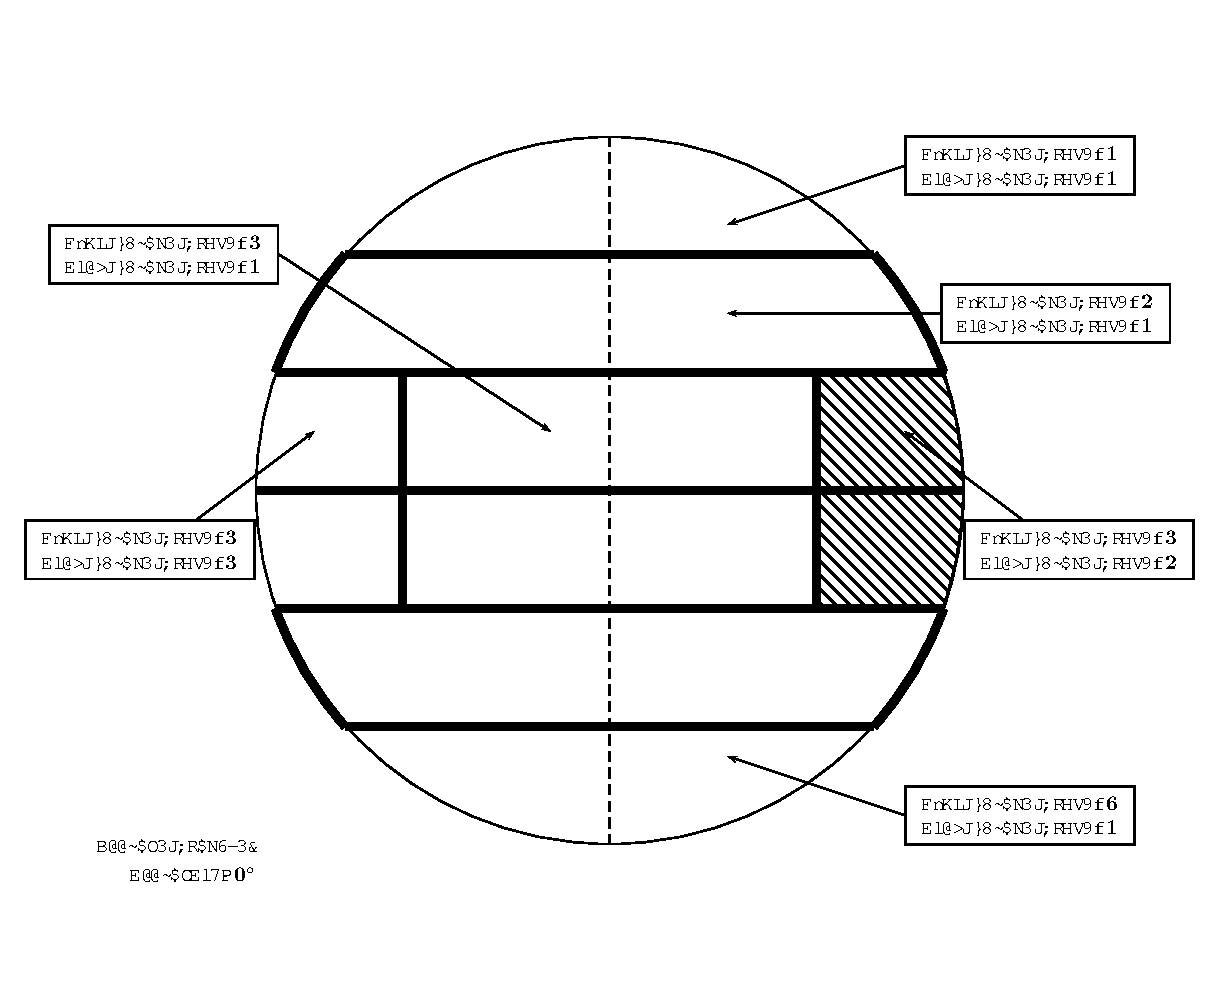
\includegraphics[width=12cm]{rgau_fig.ps}
\end{center}
\caption{適合ガウス格子の例}
\label{rgau_fig}
\end{figure}
Figure \ref{rgau_fig} のように全球を分割する場合を考える(ガウス格子では
緯度の間隔は一定ではないが、ここでは簡単にするため等間隔の場合を
考える)。全球のすべての
格子を格納する場合は、SUBC RGAU に設定する値は 

\noindent
{\tt j = 6}, {\tt j\_start = 1}, {\tt j\_n = 6}, \\
{\tt i(1) = 1}, {\tt i(2) = 2}, {\tt i(3) = 3}, {\tt i(4) = 3}, 
{\tt i(5) = 2}, {\tt i(6) = 1},\\ 
{\tt i\_start(1) = 1}, {\tt i\_start(2) = 1}, {\tt i\_start(3) = 1}, \\
{\tt i\_start(4) = 1}, {\tt i\_start(5) = 1}, {\tt i\_start(6) = 1}, \\
{\tt i\_n(1) = 1}, {\tt i\_n(2) = 2}, {\tt i\_n(3) = 3}, {\tt i\_n(4) = 3}, 
{\tt i\_n(5) = 2}, {\tt i\_n(6) = 1},\\ 
{\tt lat(1) = 75.0}, {\tt lat(2) = 45.0}, {\tt lat(3) = 15.0}, 
{\tt lat(4) = -15.0}, {\tt lat(5) = -45.0}, {\tt lat(6) = -75.0}\\
とする。このとき、データは1次元配列に
\begin{center}
\begin{tabular}{|c|c|c|c|c|c|c|c|c|c|c|c|c|c|} \hline
(1,1) & (1,2) & (2,2) & (1,3) & (2,3) & (3,3) &
(1,4) & (2,4) & (3,4) & (1,5) & (2,5) & (1,6)\\ \hline
\end{tabular} 
\end{center}
のように格納する。

Figure \ref{rgau_fig} の斜線部分のみを格納する場合は\\
{\tt j = 6}, {\tt j\_start=3}, {\tt j\_n = 2}, \\
{\tt i(1) = 1}, {\tt i(2) = 1}, \\
{\tt i\_start(1) = 2}, {\tt i\_start(2) = 2}, \\
{\tt i\_n(1) = 1}, {\tt i\_n(2) = 1}, \\
{\tt lat(1) = 15.0}, {\tt lat(2) = -15.0}, \\
とする。このとき、データは1次元配列に
\begin{center}
\begin{tabular}{|c|c|} \hline
(2,3) & (2,4)\\ \hline
\end{tabular} 
\end{center}
のように格納する。

\section{メルカトル図法 (MR)}

\paragraph{表式}
メルカトル図法 Mercator projection は
世界地図などによく用いられる円筒図法で正角図法でもある。
気象庁では一部の FAX 図や低緯度の台風モデル%
\footnote{
	台風モデルは中緯度ではランベルト正角円錐図法となり、
	事前に投影法が定めがたいため、
	データセット種別名では {\tt \_TYMXXET} などのように {\tt XX} を用いる。
}などで用いられている。

投影の表式は次のようである%
\footnote{
	巷間よく行われる説明では地球中心に光源を置き
	地球に巻きつけた円筒に写る像だといっているが
	あれは子供だましで正角図法にはならない。
	正しくは経線等間隔を仮定して
 	\EqRef{eq:conformal}
	を南北に積分する。
}:
\begin{eqnarray}
 (x - x_0) D_X &=& R (\lambda - \lambda_0)
\\
 (y - y_0) D_Y &=&
 	R \ln\left[\tan\left(\frac{\pi}{4} + \frac{\varphi}{2}\right)\right]
 	-R \ln\left[\tan\left(\frac{\pi}{4} + \frac{\varphi_0}{2}\right)\right]
\\
	&=& R \tanh^{-1}(\sin\varphi)
	- R \tanh^{-1}(\sin\varphi_0)
\\
 R &=& a\cos\varphi_1
\end{eqnarray}
ただしここで \(\tanh^{-1}\) は \(\tanh\) の逆関数であり逆数ではない。

\paragraph{定義ファイル}
この投影を決定するために必要なパラメタは
参照格子点 \(x_0\), \(y_0\),
参照経緯度 \(\lambda_0\), \(\varphi_0\),
格子間隔 \(D_X\), \(D_Y\) (メートル単位, \(D_i\) などと混同しないように)
および標準緯度%
\footnote{
	$D_X$ は標準緯度における東西方向の長さである。
}%
\(\varphi_1\)
であり、定義ファイルに次のように書かれる。
\begin{quote}
\begin{tabular}{lllll}
{\tt distance}	& $D_X$ & $D_Y$ & & \\
{\tt basepoint}	& $x_0$ & $y_0$	& $\lambda_0${\tt E} & $\varphi_0${\tt N} \\
{\tt standard}	& {\tt 0E} & $\varphi_1${\tt 0N} & {\tt 0E} & {\tt 0N} \\
\end{tabular}
\end{quote}

\paragraph{パラメタの許容範囲}
投影法は
\(-90^\circ < \varphi_1 < 90^\circ\),
\(D_X \ne 0\),
\(D_Y \ne 0\)
を要請する。
また NuSDaS インターフェイスによって
\(0 \le |\lambda_0| < 180^\circ\),
が要請される。
理論上何ら悪いことはないのだが、
\(|D_X| < 180\)m
または
\(|D_Y| < 180\)m
という場合は経緯度格子と間違えている可能性が高いので、
エラーではないが警告が表示される。

\section{ポーラーステレオ図法 (PS)}

\paragraph{表式}
ポーラーステレオ図法 polar stereographic projection は
高緯度の天気図や航空向け GPV プロダクトなどに用いられる方位図法で
正角図法でもある。
表式は次のようである。
\begin{eqnarray}
 (x - x_0) D_X &=& R \sin(\lambda-\lambda_1) - R_0 \sin(\lambda_0-\lambda_1)
\\
 (y - y_0) D_Y &=& R \cos(\lambda-\lambda_1) - R_0 \cos(\lambda_0-\lambda_1)
\\
 R &=& a(1 + \sin\varphi_1) \tan \frac{\frac{\pi}{2} - \varphi}{2}
\\
 R_0 &=& a(1 + \sin\varphi_1) \tan \frac{\frac{\pi}{2} - \varphi_0}{2}
\end{eqnarray}
参照点への平行移動や標準緯度 \((\varphi_1)\) による縮尺調整の関係で式が長いが、
要は極からの半径が \(a(1 + \sin\varphi_1)\tan[\frac{1}{2}(\frac{\pi}{2} - \varphi)]\) 
といっているに過ぎない。
南極に光源を置いて北極に接するように置いた平面に映る影が
ステレオ図法だと説明されることが多いが、
ポーラーステレオについては間違っていない%
\footnote{ヒントは円周角の定理}%
。
ここで標準緯度とは、縮尺を変えない円周を与える緯度であり、つまり投影面を置く緯度に他ならない。

\paragraph{定義ファイル}
投影を同定するのに必要なパラメタは
\((x_0, y_0)\),
\((\lambda_0, \varphi_0)\)
および標準緯度 \(\varphi_1\) と標準経度 \(\lambda_1\) であり
定義ファイルに次のように書かれる。
\begin{quote}
\begin{tabular}{lllll}
{\tt distance}	& $D_X$ & $D_Y$ & & \\
{\tt basepoint}	& $x_0$ & $y_0$	& $\lambda_0${\tt E} & $\varphi_0${\tt N} \\
{\tt standard}	& $\lambda_1${\tt E} & $\varphi_1${\tt N} & {\tt 0E} & {\tt 0N} \\
\end{tabular}
\end{quote}
次の例は標準緯度 $60^\circ$N で $140^\circ$E が $y$ 軸になる
ように投影した面の中で
40km 間隔 $83\times 71$ 格子の (65, 53) が ($30^\circ$N, $140^\circ$E) に
来るように配置したものを意味する。
\begin{screen}
\begin{verbatim}
size        83   71
basepoint   65.0   53.0   140.0E  30.0N
distance    40000.0  40000.0
standard    140.0E 60.0N 0.0E 0.0N
\end{verbatim}
\end{screen}

\paragraph{パラメタの許容範囲}
投影法は
\(0 < |\varphi_1| < 90^\circ\),
\(D_X \ne 0\),
\(D_Y \ne 0\)
を要請する。
NuSDaS インターフェイスは
メルカトル図法のチェックに加えて
\(|\lambda_1| \le 180^\circ\)
を要請する。

\section{ランベルト正角円錐図法 (LM)}

\paragraph{表式}
ランベルト正角円錐図法 Lambert conformal conic projection 
(正角割円錐図法 などいろいろに呼ばれる)
はポーラーステレオに比べれば中緯度での縮尺の変動が小さい円錐図法で、
正角図法であることから中緯度の天気図や領域モデルによく用いられる。

\begin{eqnarray}
 (x - x_0) D_X
 &=&
 R\sin[n(\lambda - \lambda_1)]
 - R_0\sin[n(\lambda_0 - \lambda_1)]
 \label{eq:lambert:first}
\\
 (y - y_0) D_Y
 &=&
 R\cos[n(\lambda - \lambda_1)]
 - R_0\cos[n(\lambda_0 - \lambda_1)]
\\
 R
 &=&
 F \tan^{n} \left(\frac{\frac{\pi}{2} - \varphi}{2}\right)
\\
 R_0
 &=&
 F \tan^{n} \left(\frac{\frac{\pi}{2} - \varphi_0}{2}\right)
\\
 F
 &=&
 \frac{a}{n} \cos\varphi_1
 \tan^{-n} \left(\frac{\frac{\pi}{2} - \varphi_1}{2}\right)
 \nonumber
\\
 &=&
 \frac{a}{n} \cos\varphi_2
 \tan^{-n} \left(\frac{\frac{\pi}{2} - \varphi_2}{2}\right)
\\
 n
 &=&
 \frac{ \ln\cos\varphi_1 - \ln\cos\varphi_2 }%
 {
	\ln\tan\left(\frac{\frac{\pi}{2} - \varphi_1}{2}\right)
	- \ln\tan\left(\frac{\frac{\pi}{2} - \varphi_2}{2}\right)
 }
 \label{eq:lambert:last}
\end{eqnarray}

なお、
\(\varphi_1 = \varphi_2\)
の特殊な場合は \EqRef{eq:lambert:last} は
零割る零になってしまうので
計算できず、かわりに極限である
\(
n = \sin\varphi_1
\)
とする。

\paragraph{定義ファイル}
この投影法を同定するために必要なパラメタは
\(x_0, y_0\),
\(\lambda_0, \varphi_0\),
および 標準経度
\(\lambda_1\)
と 2 つの標準緯度
\(\varphi_1, \varphi_2\),
であり、定義ファイルには次のように書かれる ($\lambda_1$ は重出)。
\begin{quote}
\begin{tabular}{lllll}
{\tt distance}	& $D_X$ & $D_Y$ & & \\
{\tt basepoint}	& $x_0$ & $y_0$	& $\lambda_0${\tt E} & $\varphi_0${\tt N} \\
{\tt standard}	& $\lambda_1${\tt E} & $\varphi_1${\tt N} &
	$\lambda_1${\tt E} & $\varphi_2${\tt N} \\
\end{tabular}
\end{quote}

次の例は RSM で用いられているもので、
標準緯度 ($30^\circ$N, $60^\circ$N) として
$140^\circ$E が $y$ 軸となるように投影した
面の中で 20km 間隔 $325\times 257$ 格子の (200, 185) が
($30^\circ$N, $140^\circ$E) に来るように配置したものを意味する。

\begin{screen}
\begin{verbatim}
size        325 257
basepoint   200.  185.  140.0E  30.0N
distance    20000. 20000.
standard    140.0E  30.0N 140.0E  60.0N
\end{verbatim}
\end{screen}

\paragraph{パラメタの許容範囲}
投影法が
\(0 < |\varphi_1| \le |\varphi_2| < 90^\circ\),
\(\varphi_1\varphi_2 > 0\),
\(D_X \ne 0\),
\(D_Y \ne 0\)
を要請する。
NuSDaS インターフェイスは
{\bf ポーラーステレオの条件に加えて}
上のチェックを行う。

\section{斜軸ランベルト図法 (OL)}
\label{sec:proj:OL}

\paragraph{表式}
斜軸ランベルト図法は基本的に上述のランベルト図法の投影中心を北極から
中緯度の適当な地点に移したもので、マップファクターの等しい線が緯線ではなく
経線・緯線と斜めに交わる任意の小円に設定できて、
日本列島のように描画対象が弧状に存在している場合に図全体での
縮尺の差を小さくすることができることに意義がある。
ただし地球の楕円体性の考慮の方式にいろいろあり、
単に斜軸ランベルトというだけでは具体的地図投影写像はひとつには決まらない。

経緯度から地図座標への変換は大きく分けて3段階からなる。
\begin{itemize}
\item
	回転楕円体等角写像
\item
	斜軸回転
\item
	ランベルト正角円錐図法
\end{itemize}

まず回転楕円体等角写像は
回転楕円体上の点\footnote{
	一般に用いられる経緯度は回転楕円体上の経緯度である。
}
\((\lambda, \varphi)\)
を球面上の点
\((\hat{\lambda}, \hat{\varphi})\)
に対応付けるもので、次のようなものである:
\begin{eqnarray}
 \hat{\lambda} &=& c(\lambda - \lambda_E) + \lambda_E
 \label{eq:gauss-aposphere:lon}
\\
 \hat{\varphi} &=&
	2\tan^{-1} \left[
		\tan \frac{\frac{\pi}{2} + \varphi}{2}
		\left(
			\frac{1 - e\sin\varphi}{1 + e\sin\varphi}
		\right)^{\frac{e}{2}}
	\right]^{c}
	- \frac{\pi}{2}
 \label{eq:gauss-aposphere:lat}
\\
 c &=& \sqrt{
   \frac{1 + e^2\cos^4(\varphi_E)}{1 - e^2}
 \label{eq:gauss-aposphere:last}
 }
\end{eqnarray}
ここでパラメタ $e$ は回転楕円体の離心率と呼ばれ
GRS80 系の $0.081819218$ が用いられる。
なお、Snyder \cite{snyder} によれば
\begin{eqnarray}
	\hat{\lambda} &=& \lambda
	\label{eq:snyder-aposphere:lon}
\\
	\hat{\varphi} &=&
	2\tan^{-1} \left[
		\tan \frac{\frac{\pi}{2} + \varphi}{2}
		\left(
			\frac{1 - e\sin\varphi}{1 + e\sin\varphi}
		\right)^{\frac{e}{2}}
	\right]
	- \frac{\pi}{2}
	\label{eq:snyder-aposphere:lat}
\end{eqnarray}
のようにしても等角写像を得ることができて、
もちろんこのほうが2つのパラメタが不要で
簡単だし全球が写像できるメリットもあるのだが
座標値が 10km 単位でずれるので
数値予報標準ライブラリ以外の方法で地図投影している
GIS ソフトウエアの利用にあたっては注意を要する。

次に行われる斜軸回転とは、
正軸球座標における (\(\hat{\lambda}_P, \hat{\varphi}_P\)) を
新座標における北極 (\(\varphi' = \pi/2\)) に対応付け、
正軸球座標における北極を新座標における経度ゼロとするような
新しい球座標 (\(\lambda', \varphi'\)) であり、
次のような式が用いられている。
\begin{eqnarray}
 \varphi' &=& \sin^{-1}\left[
 	\sin\hat{\varphi}_P\sin\hat{\varphi}
 	+ \cos\hat{\varphi}_P\cos\hat{\varphi}
	\cos(\hat{\lambda} - \hat{\lambda}_P)
	\right]
 \label{eq:rotate:lat}
\\
 \lambda' &=& \tan^{-1}\frac{
 	\cos\hat{\varphi}\sin(\hat{\lambda} - \hat{\lambda}_P)
 }{
 	\cos\hat{\varphi}_P\sin\hat{\varphi}
	- \sin\hat{\varphi}_P\cos\hat{\varphi}
	\cos(\hat{\lambda} - \hat{\lambda}_P)
 }
 \label{eq:rotate:lon}
\end{eqnarray}
この変換は地軸に関する経度方向の $\hat{\lambda}_P$ 回転と
東経 90 度軸に関する
\(
 \hat{\theta}_P = \frac{\pi}{2} - \hat{\varphi}_P
\)
だけの回転の合成であるはずだから
\begin{eqnarray*}
 \pmatrix{
  \cos\varphi'\cos{\lambda}' \cr
  \cos\varphi'\sin{\lambda}' \cr
  \sin\varphi' \cr
 }
 &=&
 \pmatrix{
  \cos\hat{\theta}_P & 0 & -\sin\hat{\theta}_P \cr
  0 & 1 & 0 \cr
  \sin\hat{\theta}_P & 0 & \cos\hat{\theta}_P \cr
 }
 \pmatrix{
  \cos\hat{\lambda}_P & \sin\hat{\lambda}_P & 0 \cr
  -\sin\hat{\lambda}_P & \cos\hat{\lambda}_P & 0 \cr
  0 & 0 & 1 \cr
 }
 \pmatrix{
  \cos\hat{\varphi}\cos\hat{\lambda} \cr
  \cos\hat{\varphi}\sin\hat{\lambda} \cr
  \sin\hat{\varphi} \cr
 }
\\
 &=&
 \pmatrix{
  \sin\hat{\varphi}_P \cos\hat{\varphi} \cos(\hat{\lambda} - \hat{\lambda}_P)
  - \cos\hat{\varphi}_P \sin\hat{\varphi}
  \cr
  \cos\hat{\varphi} \sin(\hat{\lambda} - \hat{\lambda}_P)
  \cr
  \cos\hat{\varphi}_P \cos\hat{\varphi} \cos(\hat{\lambda} - \hat{\lambda}_P)
  + \sin\hat{\varphi}_P \sin\hat{\varphi}
  \cr
 }
\end{eqnarray*}
となるが、\EqRef{eq:rotate:lon} の \(\lambda'\) と符号が逆であるから
\(\lambda'\) は西経が正となっていることを意味する。

最後のランベルト正角円錐図法による地図投影は、
式 \ref{eq:lambert:first}--\ref{eq:lambert:last} の
経緯度
\(\lambda', \varphi'\)
に斜軸球面経緯度
\(\lambda', \varphi'\)
をあてはめればよいが、次のようなことに注意されたい。
\begin{itemize}
\item
	パラメタ、特に \(\lambda_1\) は斜軸座標の値である
\item
	気象庁の斜軸ランベルトでは
	極から参照点に向かう軸 (南東向き) を $x$,
	それに右向き直交する軸 (南西向き) を $y$ としているので
	式 \ref{eq:lambert:first}--\ref{eq:lambert:last} の
	$x, y$ を入れ換えたものにあたる
\end{itemize}

\paragraph{定義ファイル}

この投影法を同定するために必要なパラメタは正軸ランベルトのパラメタに加えて
斜軸回転のパラメタ
\(\hat\lambda_P, \hat\varphi_P\),
と楕円体等角写像のパラメタ
\(\lambda_E, \varphi_E\),
であり、定義ファイルには次のように書かれる。
\begin{quote}
\begin{tabular}{lllll}
{\tt distance}	& $D_X$ & $D_Y$ & & \\
{\tt basepoint}	& $x_0$ & $y_0$	& $\lambda_0${\tt E} & $\varphi_0${\tt N} \\
{\tt standard}	& $\lambda_0${\tt E} & $\varphi_1${\tt N} &
	$\lambda_0${\tt E} & $\varphi_2${\tt N} \\
{\tt others} & $\hat\lambda_P${\tt E} & $\hat\varphi_P${\tt N} &
	$\lambda_E${\tt E} & $\varphi_E${\tt N} \\
\end{tabular}
\end{quote}
STANDARD 文にも $\lambda_0$ が書かれておりランベルト投影の標準経度
\(\lambda_1\)
が独立に示されていないが、
気象庁では参照点 \(\lambda_0, \varphi_0\) を楕円体等角写像・斜軸回転
して得る斜軸経度を用いるためである。
%
次の例は 1km 格子である。
%
\begin{screen}
\begin{verbatim}
size        1600 3600
distance    1000 1000
basepoint   1053 1403 35.3572N 138.7306E
standard    45.8183N 138.7306E 50.9429N 138.7306E
others      56.1920N 82.7382E 37.0N 137.0E
\end{verbatim}
\end{screen}

\paragraph{投影法パラメタの由来}

気象庁で用いられている斜軸ランベルト図法は格子間隔と
参照点格子番号を除いて上の定義ファイル例のパラメタを用いているが、これは
国土地理院が 1972 年に発行した
300 万分の 1 「日本とその周辺」図の投影法に由来する。
\(
	\lambda_E = 137^\circ, \varphi_E = 37^\circ
\)
は別にすると
\( \hat\lambda_P = 82^\circ44'17''.4 \),
\( \hat\varphi_P = 56^\circ11'31''.3 \),
\( \varphi_1 = 45^\circ49'06''.0 \),
\( \varphi_2 = 50^\circ56'34''.4 \)
は
大変切りの悪い数値であるが、
導線 (縮尺が最小となる線で斜軸座標の緯線) が
占守島 (\(50^\circ46'\)N, \(156^\circ03'\)E)\footnote{
	占守島は幌筵島
	(32215 SEVERO-KRIL'SK 50:41N, 145:08E) より東だからこの経度は
	明らかに間違っている。
	ちなみに名古屋と台北の経緯度はちょうど 47636 と 46692 に一致する。
}
名古屋 (\(35^\circ10'\)N, \(136^\circ58'\)E),
台北 (\(25^\circ02'\)N, \(121^\circ31'\)E),
を通り、その縮尺が 0.999 となるように決められているという\cite{kanazawa}。
参照点
\(\lambda_0 = 138^\circ43'50''\),
\(\varphi_0 = 35^\circ21'26''\)
はレーダーエコー合成図に由来し、
富士山の経緯度である\cite{makihara}。

当時のことであるから (特に富士山の) 経緯度は
旧日本測地系によるものであるが、
現在でも前節の投影法パラメタを
そのままに地球の形だけ GRS80 系に変更して用いている。
理論上この斜軸座標は 2002 年 4 月 1 日の改正測量法施行時
あるいは地球の形として GRS80 系が採用された NAPS8 の移行時に
400--500m ほどシフトされたことになるが、
それが問題になるプロダクトは今のところ存在しない。

\paragraph{パラメタの許容範囲}
現在のところ正軸ランベルトと同じチェックが行われる。

\section{子午面断面図 (YP)}
\paragraph{定義ファイル}
鉛直22層、南北73格子の例を次に示す。
\begin{screen}
\begin{verbatim}
plane 1
plane1 ZONAL
size 73 22
basepoint 1 1 0E 90N
distance 2.5 2.5
\end{verbatim}
\end{screen}
\paragraph{パラメタの許容範囲}
\(0 < |D_J| < 180^\circ\),
\(|\lambda_0| \le 180^\circ\),
\(|\varphi_0| \le 90^\circ\)
が要請される。

\section{東西断面図 (XP)}

\paragraph{定義ファイル}
鉛直1層、東西360格子の例を次に示す。
\begin{screen}
\begin{verbatim}
size 360 1
basepoint 1 1 0E 0N
distance 1.0 1.0
\end{verbatim}
\end{screen}
\paragraph{パラメタの許容範囲}
\(0 < |D_I| < 180^\circ\),
\(|\lambda_0| \le 180^\circ\),
\(|\varphi_0| \le 90^\circ\)
が要請される。

\section{レーダー画像 (RD)}

\paragraph{定義}
国内二進電文の資料から察して
レーダーサイトを中心とした正距方位図法の投影面上の等間隔格子であると解されるが
投影法諸元を掲げることができるような厳密な定義は調査中である。
\paragraph{定義ファイル}
格子間隔が書かれる。
メンバー毎に違うレーダーサイトを表現する
多メンバーのデータセットにすることが多いので
参照点は書かれないのが普通である。
また、レーダーデータについては通常 \verb|value REPR| が書かれる。
\begin{screen}
\begin{verbatim}
size        200 200
distance    2500 2500
value       REPR
\end{verbatim}
\end{screen}

\paragraph{パラメタの許容範囲}
投影法は
\(D_X \ne 0\),
\(D_Y \ne 0\)
を要請する。
理論上何ら悪いことはないのだが、
\(|D_X| < 180\)m
または
\(|D_Y| < 180\)m
という場合は経緯度格子と間違えている可能性が高いので、
エラーではないが警告が表示される。
また、\DefRef{BASEPOINT} を書いた場合は経緯度が過大だとエラーになる。

\paragraph{注意}
なお、次項で述べる極座標に {\tt RD} を用いている例があるため注意を要する。
このようなデータは $D_X$ に比べて $D_Y$ だけが桁違いに小さい。

\section{レーダー極座標格子 (RT)}

\paragraph{定義}
X ($r$) 軸が距離、Y ($\theta$) 軸が方位角である。
したがって通常 $D_\theta = 360^\circ / N_Y$ である。
方位角の原点は北であると思うがデータ作成元に確認されたい
(将来の版ではこの点を明確化する必要がある)。

\paragraph{定義ファイル}
次のような形式で記述する。

\begin{quote}
\begin{tabular}{lll}
{\tt size} & $N_X$ & $N_Y$ \\
{\tt distance} & $D_r$ & $D_\theta$ \\
\end{tabular}
\end{quote}

具体例を挙げると次のようになる。

\begin{screen}
\begin{verbatim}
size        200  256
distance    1500  1.40625
value       REPR
\end{verbatim}
\end{screen}

\paragraph{パラメタの許容範囲}
投影法は
\(D_r \ne 0\),
\(0 < |D_\theta| < 180^\circ\)
を要請する。
理論上何ら悪いことはないのだが、
\(|D_r| < 180\)m
という場合は経緯度格子と間違えている可能性が高いので、
エラーではないが警告が表示される。


\section{地点 (ST)}
\paragraph{表式}
アメダスデコードについて利用されている。
この格子系のデータについては、
データ要素として経緯度
{\tt LAT},
{\tt LON},
または
{\tt MLAT},
{\tt MLON},
が格納されていなければ、
各格子点の位置についてはデータ作成元に問い合わせるほかない。
\paragraph{定義ファイル}
投影法関連の文 [\DefRef{DISTANCE} 等] は通常省略される。
\paragraph{パラメタの許容範囲}
特段のチェックは行われない。

\section{細分 (SB)}
\paragraph{表式}
検証デコードについて利用されている。
この格子系のデータについては、
データ要素として、細分番号
{\tt SB\_NUM},
が格納されていなければ、
各格子点の位置についてはデータ作成元に問い合わせるほかない。
\paragraph{定義ファイル}
投影法関連の文 [\DefRef{DISTANCE} 等] は通常省略される。
\paragraph{パラメタの許容範囲}
特段のチェックは行われない。

\section{自由格子 (FG)}
\paragraph{表式}
河川に沿った格子について利用されている。
この格子系のデータについては、
各格子点の位置についてはデータ作成元に問い合わせるほかない。
\paragraph{定義ファイル}
投影法関連の文 [\DefRef{DISTANCE} 等] は通常省略される。
\paragraph{パラメタの許容範囲}
特段のチェックは行われない。

\section{その他の格子 (XX)}
\label{sec:proj:XX}

この「座標系」は台風モデルによって用いられている。
台風モデルは台風の中心位置が低緯度のときメルカトル図法、
中緯度のときランベルト正角円錐図法となるので、
事前に種別名を定めておきたい
(あるいは、台風モデルの出力をひとつのデータセットに蓄積したい)
という目的から便宜上 {\tt XX} を用いる。
台風モデルは実行時に \APIRef{nusdas.grid}{nusdas\_grid} を用いて
投影法パラメタを設定している。

このような運用に配慮して、
2次元座標系が {\tt XX} のときは
データファイルを作成しようとするときに行われる投影法パラメタチェックが
抑止される。
そのかわり、ファイルを閉じようとするさいに依然として
投影法が {\tt XX} であれば、
nusdas\_grid を呼び忘れたものとみなしてエラーになる。

\Chapter{3次元座標系と鉛直座標パラメタ}
\label{chap:3dcoord}

\section{気圧座標 (PP)}
気圧$p$ を独立変数にした座標系である。
座標を構成するにあたって必要なパラメータはない。

面名は hPa 単位で数値を6文字の文字列(左詰めで余りには空白を埋め
る)で表す。

\section{エータ座標 (ET)}
$\sigma - p$ 座標とも呼ばれ、下層では地形に沿った$\sigma$座標系、上層で
は水平な $p$ 座標系になっている(Figure \ref{eta_full_half})。

\begin{figure}[h]
\begin{center}
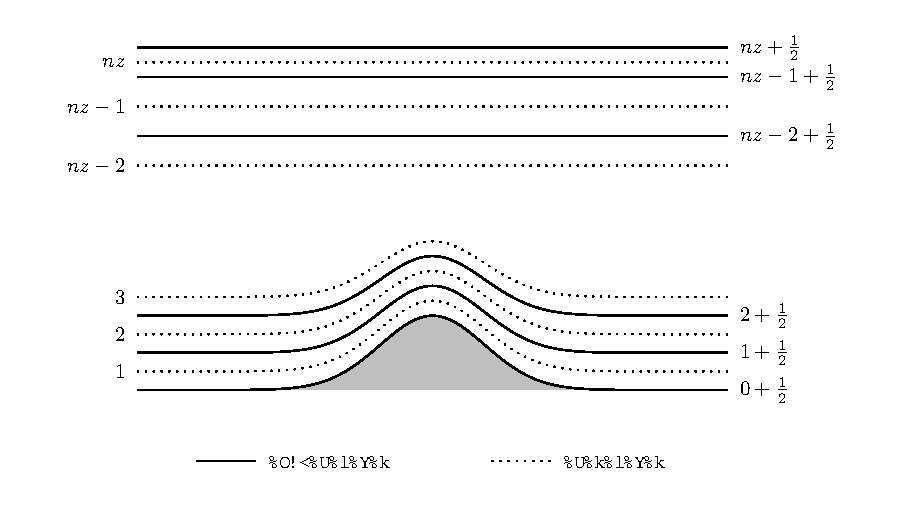
\includegraphics[height=6cm]{eta_full_half.ps}
\end{center}
\caption{エータ座標系の模式図(GSM, RSMなど)。
 地表面はハーフレベルの最下層に一致する。
 この地表面まで含めたときにハーフレベルの層数は鉛直層数(フルレベルの層数)
 より1だけ多いことに注意。そのため、ハーフレベルに対応する値を格納する
 SUBC ETA の$A$, $B$ の要素数が(鉛直層数+1)必要になる。}
\label{eta_full_half}
\end{figure}

各点の気圧は、SUBC ETA レコードに格納されている係数 $A$, $B$, $C$ を用い
て
\[
 p(x, y, z) = B(z)[p_G(x, y, z) - C] + A(z)
\]
と表現される(実際には$C=0$である)。

$A$, $B$ は、ハーフレベルに対応した値が格納されており\footnote{$p$はハー
フレベルに配置されている。}、ハーフレベルの最下層が地表面に一致するよう
になっている。また、ハーフレベルはフルレベルより1層多いので、$A$, $B$ は
鉛直層数(フルレベルの層数) に1を加えた数の配列を確保する必要がある。

データは通常、フルレベルの値が格納され、層名は下からつけた番号を
6文字の文字列(左詰めで余りには空白を埋める)で表す。

\section{シグマ座標 (SG)}
ある一定の気圧を $p_T$、地表面の気圧を $p_G$、各点の気圧を $p$ としたと
き、
\[
 \sigma(x, y, z) = \frac{p(x, y, z) - p_T}{p_G(x, y) - p_T}
\]
で定義された変数を独立変数にする座標系である。

地形に沿った座標系で、地球表面に山があっても、地表面は
$\sigma = 1$ で表される。

各点の気圧は、ETA 座標と同様に、
SUBC SIGM レコードに格納されている係数 $A$, $B$, $C$ を用い
て
\[
 p(x, y, z) = B(z)[p_G(x, y, z) - C] + A(z)
\]
と表現される($A$, $B$, $C$ については、ETA と同じ要素数を持つ配列または
変数)。
$A$が $p_T$ に、$B$ が $\sigma$ に、$C$ が $p_T$ に対応する
\footnote{$p_T$ はスカラーであるが、ETAとデータ構造を同じにするため、
配列である $A$ に格納している。格納の際には、すべての要素に同じ値を格納
するようにする。}。


データは通常、フルレベルの値が格納され、層名は下からつけた番号を
6文字の文字列(左詰めで余りには空白を埋める)で表す。

\section{ハイブリッド気圧座標 (HB)}

用例はない。名前だけ予約されていると解されたい。
鉛直座標パラメタを格納するために
SUBC ETA レコードで対応できるか否かも未定である。

\section{バイブリッド鉛直座標(Z*座標の拡張)(ZS)}
一般に、絶対高度座標 $z$ と変換した座標系の座標 $\zeta$ が
\[
 z = \zeta + z_s f(\zeta)
\]
の関係式に表される座標系である。Z*座標系($\zeta$ を $z^*$と標記する)
\[
 z^* = \frac{z_T(z-z_s)}{H-z_s}
\]
は、
\[
 f(\zeta) = 1-\frac{\zeta}{z_T}
\]
としたものである。
ここで、$z_s$ は地形、$z_T$ はモデルトップである。

運動方程式に中に現れる座標変換に伴うテンソルは
\begin{eqnarray*}
 G^{\frac12} &=& 1 + z_s f'(\zeta) \\
 G^{\frac12}G^{13} &=& -f(\zeta)\frac{\partial z_s}{\partial x} \\
 G^{\frac12}G^{23} &=& -f(\zeta)\frac{\partial z_s}{\partial y}
\end{eqnarray*}
と表現できて、高度$z$やテンソルの算出にはモデル面の高度$\zeta$、
$f(\zeta)$および$f'(\zeta)$ があればよい。

NuSDaS では SUBC ZHYB に、モデル面の高度$\zeta$を
{\tt zrp}(フルレベル)、{\tt zrw}(ハーフレベル)、$f(\zeta)$ を \newline
{\tt vctrans\_p}(フルレベル)、{\tt vctrans\_w}(ハーフレベル)、
$f'(\zeta)$ を{\tt dvtrans\_p}(フルレベル)、{\tt dvtrans\_w}(ハーフレベ
ル)として格納されている。
\section{高度による鉛直座標 (ZZ)}
(地形を考慮しない)高度を鉛直座標にとった座標系である。

\section{温位座標 (TH)}
温位を鉛直座標にとった座標系である。
用例は確立されていないが、温位がケルビン単位の整数であれば単にその値を
\verb|printf("%g")| したものを面名にするのが適当である。

\section{経度 (LO)}

二次元座標系が {\tt YP} の時に用いられる。
実際には経度の値が用いられることはなく、
東西平均 {\tt ZONAL} だけが用いられる。

そうでないときはおとなしく {\tt LL PP} を使ってもらいたい。

\section{緯度 (LA)}

二次元座標系が {\tt XP} の時に用いられるため予約された名前である。
用例はない。

\section{閾値 (TO)}
閾値を面とみなして扱うもので、実際の鉛直座標系ではない。
主に、検証で使用する。

\section{その他の鉛直座標 (XX)}

GRIB 等のデコーダで未知の座標を表現するために予約された名前であり、
積極的に使うべきでない。
